\documentclass[]{article}
\usepackage[UTF8]{ctex}
\usepackage{amsmath}

\usepackage{graphicx}
\usepackage{algorithm,algpseudocode}

\usepackage{geometry}
\geometry{
	a4paper,
	total={170mm,257mm},
	left=20mm,
	top=15mm
}
%\usepackage{algorithmic}
\numberwithin{equation}{subsection}



\title{Spam with the BERT}
\author{eggachecat}
\date{}
\begin{document}
	
	\maketitle
	
	\newcommand{\norm}[1]{\left\lVert#1\right\rVert}
	\newcommand{\abs}[1]{\lvert#1\rvert}
	
	\newcommand{\argminE}{\mathop{\mathrm{argmin}}}          % ASdeL
	\newcommand{\argminF}{\mathop{\mathrm{argmin}}\limits}   % ASdeL
	
	\section{Notes}
	\subsection{Architecture}
	\subsection{Attention}
	\subsubsection{Encoder-Decoder Attention}
		this is some nonsence
	\begin{figure}[!htb]
		\centering
		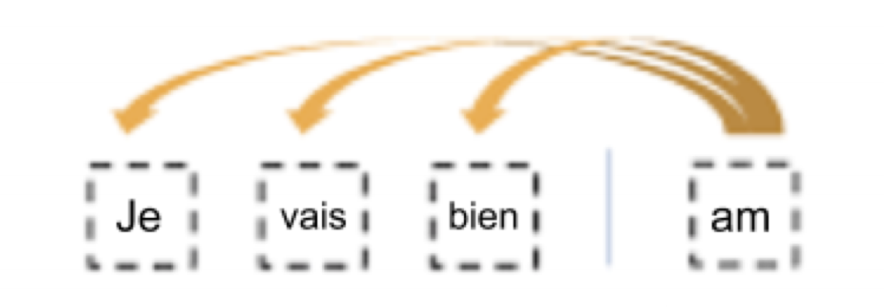
\includegraphics[width=10cm]{./assets/encoder-decoder-attention.png}
		\caption{encoder-decoder-attention}
		\label{fid:encoder-decoder-attention}
	\end{figure}
	\subsubsection{Encoder Self-Attention}
	this is some nonsence
	\begin{figure}[!htb]
		\centering
		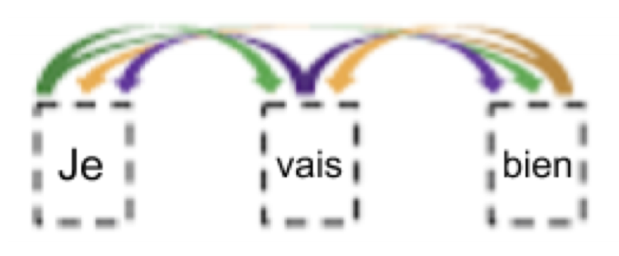
\includegraphics[width=10cm]{./assets/encoder-self-attention.png}
		\caption{encoder-decoder-attention}
		\label{fid:encoder-self-attention}
	\end{figure}
	\subsubsection{Decoder Self-Attention}
		this is some nonsence
	\begin{figure}[!htb]
		\centering
		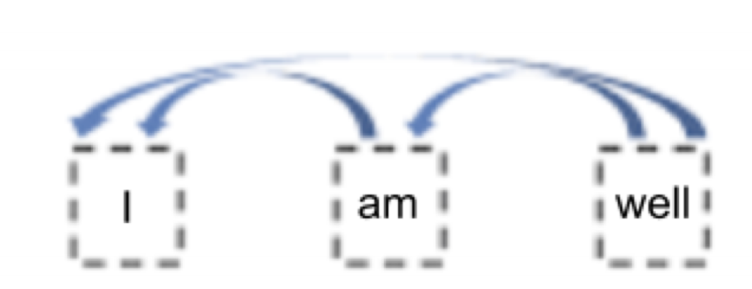
\includegraphics[width=10cm]{./assets/decoder-self-attention.png}
		\caption{encoder-decoder-attention}
		\label{fid:decoder-self-attention}
	\end{figure}
	\subsection{Masks}
	\subsection{IsNextSentence}
	
	\section{Implementation - the easy way}
	\subsection{Dependencies}
	\begin{enumerate}
		\item bert-as-service
			\begin{itemize}
				\item https://github.com/hanxiao/bert-as-service
				\item 1.6k stars <- 靠谱!
				\item 把pretrained的BERT模型host在一个http server上
				\item 易用\&易扩展
				\item 有中文的BERT的pretrained
					\begin{itemize}
						\item \textit{No, if you are using the pretrained Chinese BERT released by Google you don't need word segmentation. } -- README
						\item 意味着不用把句子分词!
					\end{itemize}
			\end{itemize}
		\item Python >= 3.5
		\item Tensorflow >= 1.10 
	\end{enumerate}
	\subsection{Datasets}
	\subsection{Traning}
	\subsubsection{预处理}
	对于一个新闻$\text{NEWS}_1$,首先分成一组句子$\text{word or phrase}$
	\begin{enumerate}
		\item 预处理
			\begin{itemize}
				\item 对于一个新闻$\text{NEWS}_1$
				\item 分成
			\end{itemize}
	\end{enumerate}
	\subsection{Inference}
	\subsection{Resultls}
	\subsection{Conclusion}
	
	
\end{document}
